\subsection{Layered protocols}
The \textit{layered protocols} are protocols in which there is a clear division between different layers. Every layer has a specific function and we can say that each layer speaks with the corresponding layer on the other side.

\subsubsection{OSI model}
An example of \textit{layered protocol} is the \textit{OSI model}. As we can see from \textit{Figure 1}, we have several levels, each of which plays a specific role. 

\begin{figure}[h]
\caption{OSI model}
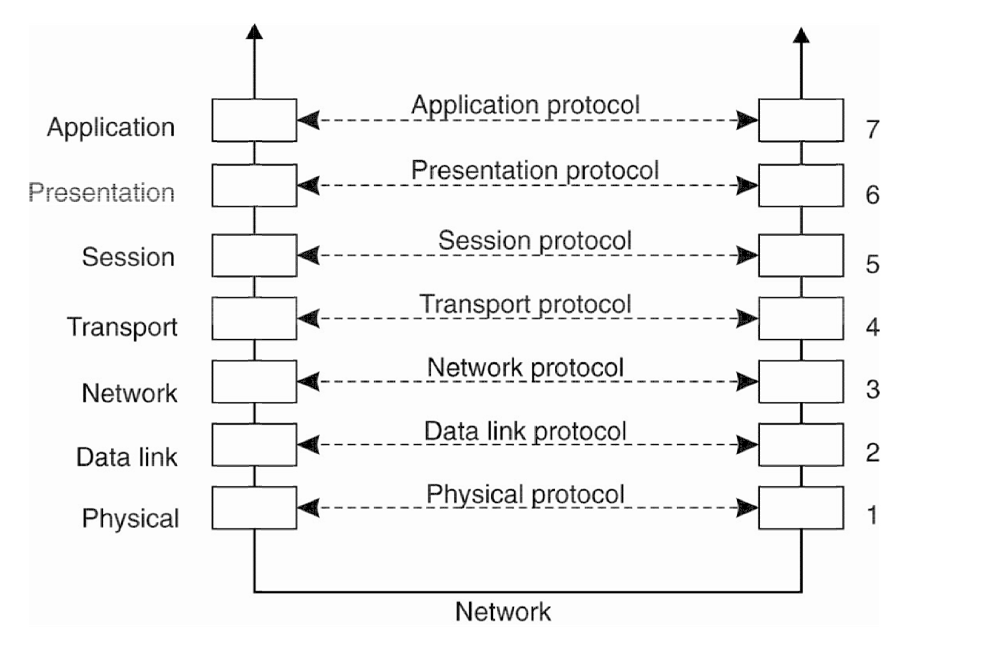
\includegraphics[width=\textwidth]{src/images/osi-model.png}
\centering
\end{figure}

In the \textit{OSI model} we distinguish between three different kinds of layers.
\begin{itemize}
    \item \textbf{Low layers}
        \begin{itemize}
            \item \textit{Physical layer}: it describes the bit transmission
            \item \textit{Data link layer}: it describes the organization of the series of bits into frames
            \item \textit{Network layer}: it describes how packets have to be routed
        \end{itemize}
    \item \textbf{Transport layer}
        \begin{itemize}
            \item It describes how data is transmitted
            \item \unserline{It offers a service independent from the lower layers}
            \item It provides the actual communication facilities for most distributed systems
        \end{itemize}
        The main standards are \textbf{TCP} \textit{(connection-oriented, reliable, stream-oriented communication)} and \textbf{UDP} \textit{(unreliable datagram communication)}
    \item \textbf{Higher level layers}\\
        They are \textit{session, presentation and application} layers and typically they are merged together.
\end{itemize}
Another important concept is the \textit{encapsulation}. As the image above can suggest, every layer is encapsulated by the lower one.

\subsubsection{Middleware as a protocol layer}
We can consider \textit{middleware} as a protocol layer in the sense that they include common services and protocols that can be used by different applications. In practice, it can:
\begin{itemize}
    \item Implement \textit{marshaling} and \textit{unmarshaling} data procedures
    \item Implement naming protocols in order to allow sharing of resources
    \item Implement security protocol for secure communication
    \item Implement scaling mechanism, such as for replication and caching
\end{itemize}

\begin{center}\rule{3in}{0.4pt}\end{center}

\subsection{Remote procedure call}
In a \textbf{local procedure call} the parameters are passed through stack. The caller writes the parameters in the stack and then call the procedure. The called simply read the parameters from the stack since the memory is shared.\\
There are different ways to pass parameters to a procedure:
\begin{itemize}
    \item \textit{By value}: C-like when passing basic data types
    \item \textit{By reference}: Java-like when passing objects
    \item \textit{By copy/restore}: it's similar but slightly different than previous one. Value is passed in and has no effect on the value of the variable passed in until the end of the function, at which point the final value of the function variable is stored in the passed in variable.\\
    The basic difference between \textit{call by reference} and \textit{copy/restore} then is that changes made to the function variable will not show up in the passed in variable until after the end of the function while call by reference changes will be seen immediately.
\end{itemize}

\begin{figure}[h]
\caption{RPC in detail}
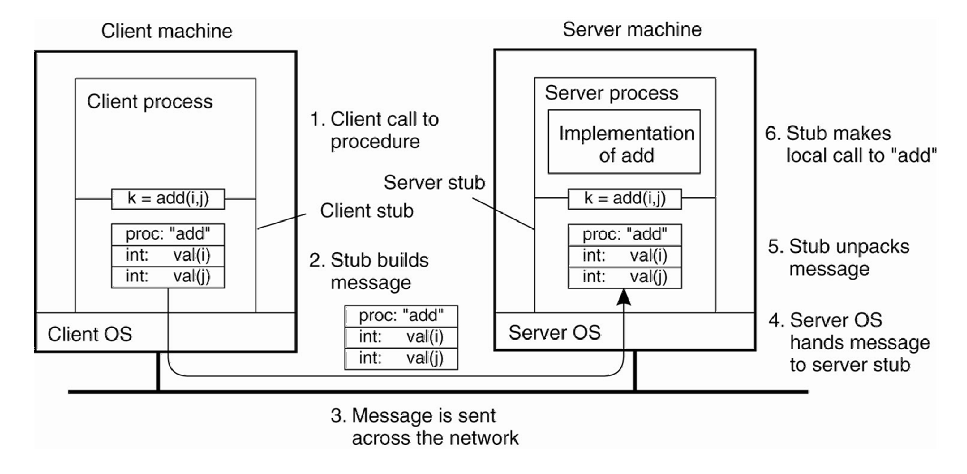
\includegraphics[width=\textwidth]{src/images/rpc-in-detail.png}
\centering
\end{figure}

\subsubsection{Marshalling and serialization}

Two problems when passing parameters:
\begin{itemize}
    \item Structured data must be ultimately flattened in a byte stream: \textbf{serialization}
    \item Hosts may use different data representations \textit{(e.g., little endian vs. big endian, EBCDIC vs. ASCII)} and proper conversions are needed: \textbf{marshalling}
\end{itemize}
In order to simplify the procedure, these operations are done by the middleware, helped by:

\begin{itemize}
    \item \textbf{IDL} \textit{(Interface Definition Language)}: a language and platform independent representation of the procedure's signature
    \begin{itemize}
        \item It raises the abstraction level of the service definition
        \item The language comes with "mappings" onto target languages
        \item It can also be used to automatically generate the service interface code in the target language 
    \end{itemize}
    \item A data representation format to be used during communication
\end{itemize}

\subsubsection{Sun Microsystems' RPC}
\begin{itemize}
    \item Also called \textit{Open Network Computing RPC}
    \item Data format is specified by \textit{XDR (eXternal Data Representation)}
    \item \textbf{Parameters are passed by value}
    \item It can use TCP or UDP
    \item Security is provided through \textit{DES}
\end{itemize}

\subsubsection{Distributed Computed Environment (DCE)}
\begin{itemize}
    \item It's a set of specifications and a reference implementation
    \item Several invocation semantics are offered
    \item Several services are provided on top of RPC
    \begin{itemize}
        \item Directory service
        \item Distributed time service
        \item Distributed file service
    \end{itemize}
    \item Security is provided through \textit{Kerberos}
\end{itemize}

\subsubsection{Binding client to server}
One of the main problems is find out which server provides a given service and how to establish communication with it and, obviously, it's undesirable to hard-writing this info in the client code.

\textbf{Sun's solution}
\begin{itemize}
    \item Introduce a daemon called \textit{portmap} that binds calls and server/ports
    \item It's important to notice that \textit{portmap} provides its services only to local clients, i.e., it solves only the problem of establish the communication
    \begin{itemize}
        \item In fact, the client must know in advance where the service resides
    \end{itemize}
    \item In order to bypass this limitation, the client can send multicast message to many \textit{portmap} daemons
\end{itemize}

\textbf{DCE's solution}
\begin{itemize}
    \item The DCE daemon works like \textit{portmap}
    \item Client doesn't need to know in advance where the service is: the only need to know where the directory service is
    \begin{itemize}
        \item The directory service can be distributed
    \end{itemize}
    \item Then, the daemon solves both the problem to find a service and establish a communication with it
\end{itemize}

\paragraph{Dynamic activation}
he server processes may remain active even in absence of requests, wasting resources. A possible solution to this problem is to introduce another (local) server daemon that:
\begin{itemize}
    \item Forks the process to serve the request
    \item Redirects the request if the process is already active
\end{itemize}
With this system, however, we have a disadvantage: the first request is served less efficiently.

\subsubsection{Lightweight RPC}
Using a conventional \textit{RPC}, sometimes, is not the better solution. For example, if we have a TCP/UDP service on the same machine a conventional \textit{RPC} would lead to wasted resources.\\
For this reason it's born the a kind of simplified \textit{RPC}, called \textit{lightweight RPC}.\\
The idea is to pass messages through local facilities, i.e. communication exploits a private shared memory region.\\
The \textit{invocation} procedure is the following:
\begin{enumerate}
    \item Client copies parameters in the shared stack and performs the system call
    \item Kernel does a context switch, to execute the procedure in the server
    \item Results are copied on the stack and another system call
    \item Context switch brings execution back to the client
\end{enumerate}
With this procedure the main advantage is that we use less threads/processes (no need to listen on a channel).

\subsubsection{Async RPC}
In a parallel system (or, more in general, in a non-distributed system), when a call is performed, the caller is suspended until the callee is done. \textit{RPC} preserves this behaviour but it can, potentially, wastes client resources.
For this reason we introduce the \textit{Async RPC}, in which the caller is not suspended and it can continue in other operations.\\
There are many variant of \textit{async RPC}:
\begin{itemize}
    \item If no result is needed execution can resume after an \textit{ack message} is received from the server
    \begin{figure}[h]
        \caption{Asynchronous}
        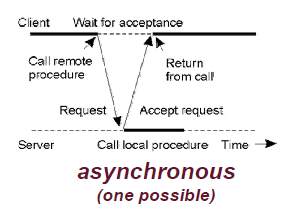
\includegraphics[scale=0.6]{src/images/async.png}
        \centering
    \end{figure}

    \item The callee may (async) invoke the caller back or invocation may return immediately a \textit{promise}
    \begin{figure}[h]
        \caption{Deferred synchronous}
        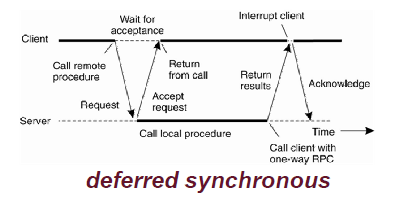
\includegraphics[scale=0.6]{src/images/deferred-synchronous.png}
        \centering
    \end{figure}
\end{itemize}

\subsubsection{Batched vs. queued RPC}
\textit{Sun RPC} includes the ability to perform \textit{batched RPC}. RPCs that do not require a result are buffered on the client and they are sent all together when a non-batched call is required or when a timeout expires. It's important to notice that this mechanism enables yet another form of \textit{async RPC}.

\subsection{Remote method invocation}

It's an approach similar to the RPC, but it aims to obtain the advantages of OOP also in the distributed setting. The main difference is that remote object references can be passed around, so need to maintain the aliasing relationship.\\
\textbf{Note that:} sometimes, this mechanism is built on top of RPC layer.

\paragraph{IDL}
The \textit{IDL} for distributed objects are much richer because it contains also inheritance, exception handling and so on.

\subsubsection{Implementation}
In practice there are two main approaches:

\begin{itemize}
\item \emph{Java RMI}: single language/platform
\begin{itemize}
    \item Easily supports passing parameters \textit{by reference} or \textit{by value} even in case of complex object
    \item Support for code on demand (downloading code)
\end{itemize}

\item \emph{OMG CORBA}: multilanguage/multiplatform
    \begin{itemize}
        \item It supports passing parameters \textit{by reference} or \textit{by value}
        \begin{itemize}
            \item If the objects are passed by value, it's up to the programmer to guarantee the same semantics for methods on the   sender and receiver sides
        \end{itemize}
    \end{itemize}
\end{itemize}

\begin{center}\rule{3in}{0.4pt}\end{center}

\subsection{Message oriented communication}

Since \textit{RPC/RMI} fosters a sync model, this approach supports only point-to-point interaction. Moreover, synchronous communication is expensive and leads to \textit{rigid} architectures, since there is an intrinsically tight coupling between caller and callee.

For this reason, there is another approach called \textbf{message oriented communication} that aims to solve these problems. In particular, it is:

\begin{itemize}
    \item centered around the notion of one-way message/event
    \item usually asynchronous
    \item often supporting persistent communication
    \item often supporting multi-point interaction
    \item brings more decoupling among components
\end{itemize}

\subsubsection{Communication types}

\begin{itemize}
    \item Sync vs. Async
    \begin{itemize}
        \item \textit{Sync}: the sender is blocked until the recipient has stored the message
        \item \textit{Async}: the sender can continues immediately after sending the message
    \end{itemize}

    \item Transient vs. persistent
    \begin{itemize}
        \item \textit{Transient}: sender and receiver must both be running for the message to be delivered
        \item \textit{Persistent}: the message is stored in the communication system until it can be delivered
    \end{itemize}
\end{itemize}

\begin{figure}[h]
    \caption{Transient communication}
    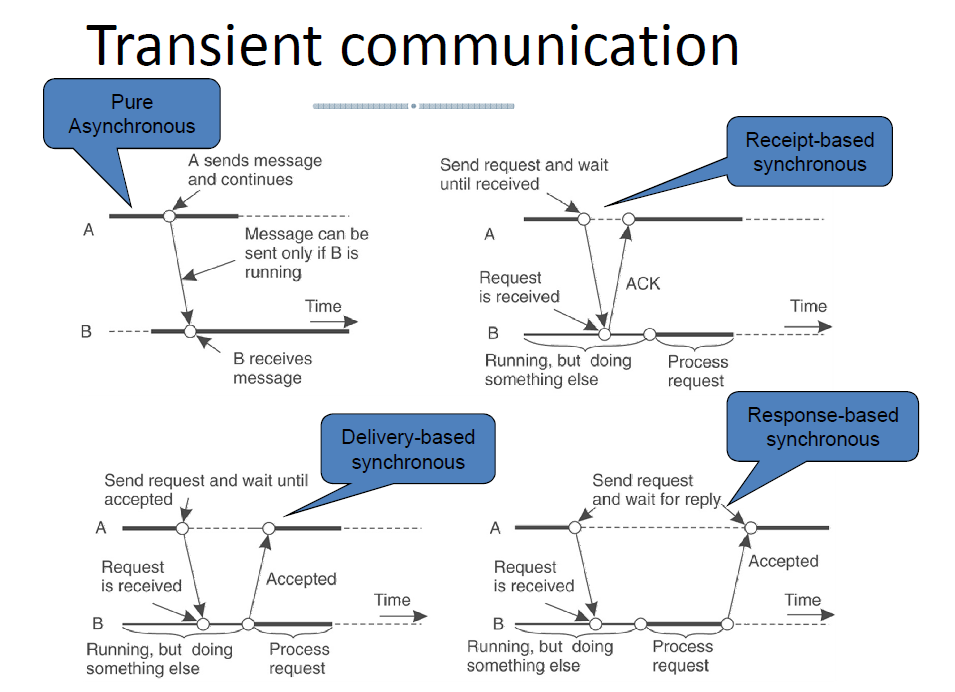
\includegraphics[width=\textwidth]{src/images/transient-communication.png}
    \centering
\end{figure}

\subsubsection{From network protocols to communication services}

Since \textit{TCP} and \textit{UDP} are well known network protocols, the question is how to take advantages from these protocols. The answer is called \textbf{Socket}.\\
Sockets provide a common abstraction for inter-process communication, and allows for connection-oriented (\textit{TCP}) or connectionless (\textit{UDP}) communication.

\paragraph{Stream socket}

It's based on concept of connection. In fact, the server accepts connection on a port and the client connects to the server. Each connected socket is uniquely identified by 4 numbers.

\paragraph{Datagram socket}

It's based on \textit{UDP}, so connectionless. Client and server use the same approach to send and receive datagrams, therefore both create a socket bound to a port and use it to send and receive datagrams.\\
There is no connection and the same socket can be used to send (or receiver) datagrams to (or from) multiple hosts.

\paragraph{Multicast socket}

It exploits the IP multicast protocol that allows to efficiently deliver \textit{UDP} diagrams to multiple recipients.\\
Component interested in receiving multicast datagrams addressed to a specific group must join the group. It's important to notice that groups are open, so it's not necessary to be a member of a group in order to send datagrams to the group.\\
Usually, it's necessary to specify a port, in order to help operating systems to decide which process on the local machine to route packets to.

\paragraph{MPI}

The sockets are protocol independent and has low level primitives.\\
This is not optimal when we are handling high performance network \textit{(e.g. clusters of computers)} where we need higher level primitives providing difference services besides pure read and write.\\
The \textbf{MPI} is born as answer to this need.
\begin{itemize}
    \item Communication take place within a known group of processes
    \item Each process within a group is assigned a local \emph{id}
    \item Messages can be sent unicast or multicast (calling the entire group)
\end{itemize}
There is no support for fault tolerance, in fact crashes are supposed to be fatal.

\subsubsection{Message Queuing}\label{message-queuing}

In point-to-point persistent async communication we need to keep track of the messages received when we weren't running.\\
For this reason we must keep a queue containing the messages received, that typically guarantee only eventual insertion in the queue, so it doesn't guarantee the recipient's behaviour.\\
It's an intrinsically peer-to-peer architecture and each component holds an input and an output queue.

\paragraph{Client-server with queues}

We can apply this approach also to client-server architecture, where the server offers a queue in which clients put their requests. The server asynchronously fetches requests, processes them and returns results in the clients' queues.\\
In this way, clients need not remain connected and queues can be shared in order to simplifies load balancing.

\paragraph{Issues and solutions}\label{issues-and-solutions}

\begin{itemize}
    \item  Since queues are identified by symbolic names, it's necessary to have a lookup service to convert queue-level addresses in network addresses.
    \item Queues are handled by queue managers, so they acting as relays
    \item Relays are often organized in an overlay network, so the messages are routed by using application-level criteria. In this way we can improve also fault tolerance.
    \item When integrating sub-systems, message conversion may be a problem. Message brokers can do this, providing application-level gateways supporting message conversion.
\end{itemize}

\subsubsection{Publish-subscribe}

The idea is that application components can publish asynchronous event notifications, and/or declare their interest in event classes by issuing a subscription.\\
\textit{Subscriptions} are collected by an event dispatcher component, responsible for routing events to all matching subscribers and collecting subscriptions. It can be centralized or distributed (for scalability reasons).
\textbf{Communication is:}
\begin{itemize}
    \item Transiently async
    \item Implicit
    \item Multipoint
\end{itemize}
\textbf{Characteristics:}
\begin{itemize}
    \item Easy to add and remove components
    \item Appropriate for dynamic \textbf{environments}
\end{itemize}
\textbf{Expressiveness} of the subscription language:
\begin{itemize}
    \item \emph{Subject-based:} the set of subjects is determined a priori
    \item \emph{Content-based:} subscriptions contain expressions that allow clients to filter events based on their content, and the set of filters is determined by client subscriptions.
\end{itemize}

\textbf{Note that:} \emph{Subject-based} and \emph{Content-based} can be combined.

\paragraph{Dispatcher}

In a distributed architecture, the dispatcher is composed by a set of message brokers organized in an overlay network which cooperate to collect subscriptions and route messages. The topology of the network may vary: \emph{acyclic vs cyclic}

\begin{itemize}
    \item In an acyclic graph:
        \begin{itemize}
            \item The messages are forwarded from broker to broker and delivered to clients only if subscribed
            \item The subscribes are forwarded from broker to broker and they are sent only once in a link
            \item The performance depends also from the forwarding algorithm used because each time a broker receives a message it   must match it against the list of received filters to determine the list of recipients
        \end{itemize}
    
    \item In a cyclic graph:
    \begin{itemize}
        \item We can use a \emph{DHT based approach}
        \item \emph{Content-based} routing, in which every source define a shortest path tree
    \end{itemize}
\end{itemize}

\subparagraph{Hierarchical forwarding}

It exploits the tree properties. In particular:
\begin{itemize}
    \item Both messages and subscriptions are forwarded by brokers towards the root of the tree
    \item Messages flow \textit{downwards} only if a matching subscription had been received along that route
\end{itemize}

\subparagraph{Complex event processing}
\textit{CEP} systems adds the ability to deploy rules that describe how composite events can be generated from primitive (or composite) ones.

\begin{center}\rule{3in}{0.4pt}\end{center}

\subsection{Stream-oriented communication}

The main concept is to send a sequence of data units in an orderly and fast way.\\
Transmission modes:
\begin{itemize}
    \item \textit{Async}: the data items in a stream are transmitted on after the other without any further timing constrains
    \item \textit{Sync}: there is a max end-to-end delay for each unit in the data stream
    \item \textit{Isochronous}: there is a max and min end-to-end delay
\end{itemize}
It needs some non-functional requirements \emph{QoS}:
\begin{itemize}
    \item Required bit rate
    \item Maximum delay to setup the session
    \item Maximum end-to-end delay
    \item Maximum variance in delay (\textit{jitter})
\end{itemize}
We can also enforcing \emph{QoS} at the application layer:
\begin{itemize}
    \item Buffering: control \textit{max jitter} by sacrificing session setup time
    \item Forward error connection
    \item Interleaving data: to mitigate the impact of lost packets
\end{itemize}
